\section{Experimental Results}

In this section we discuss our experimental evaluation.
First we describe the benchmarks with datasets used in the experiments.
Afterwards, we discuss our results concerning the instrumentations for profiling our work metric.
Finally we present the results of the online {\itercomp}.

\subsection{Evaluation of the Instrumentation}

We first compare static aspects of the instrumentation algorithms.
The naive instrumentation always has 100\% of the basic blocks instrumented, by definition.
First, we evaluate the optimal work profiling compared to the relaxation algorithm applied per DAG.
Afterwards, we compare these profiling techniques with the whole program relaxation.

Figure~\ref{fig:num-probes} shows the percentage of instrumented basic blocks for the optimal and the relaxed instrumentation with different relaxation thresholds.
While Figure~\ref{fig:num-probes} compares the various instrumentation algorithms in respect of the naive instrumentation, Figure~\ref{fig:num-probes-improvement} shows the improvement of the relaxation algorithm  over the optimal instrumentation.

%\begin{figure*}[ht]
%    \centering
%    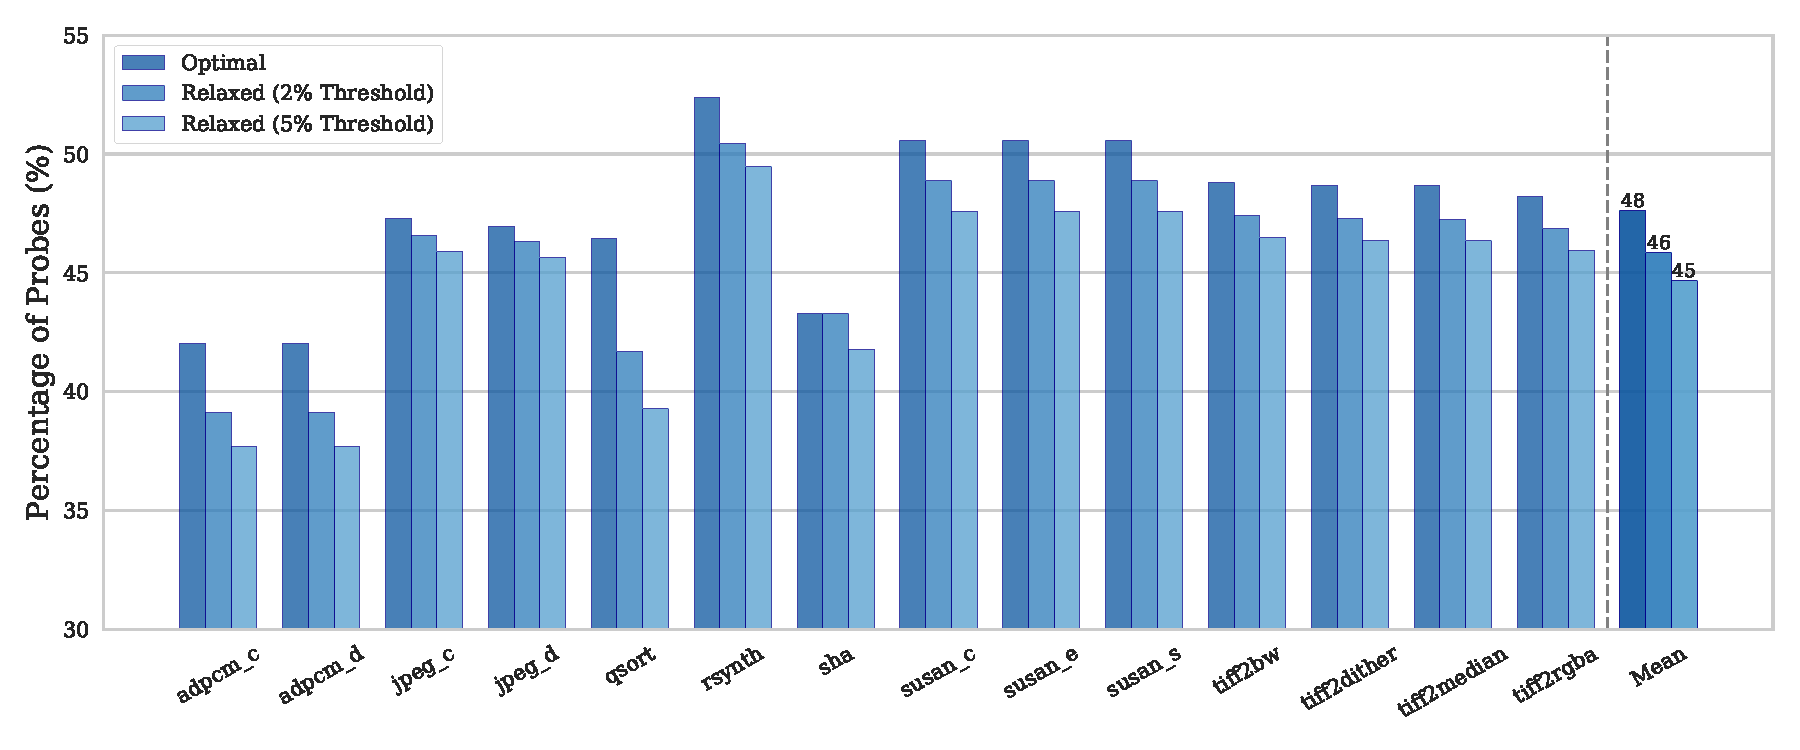
\includegraphics[width=\textwidth]{figs/num-probes.pdf}
%    \caption{Percentage of instrumented basic blocks for the optimal and the relaxed instrumentation with different relaxation thresholds.}
%    \label{fig:num-probes}
%\end{figure*}

For the evaluation of the performance overhead that the instrumentation incur to the benchmarks, we measure the wall-clock time of the benchmarks when compiled with the default {\flagstype -O3} optimization.
For each benchmark, we compute the average overhead over all its 1000 input dataset.
When measuring the wall-clock time for each input, in order to reduce noise, we execute the same input until we have a statistically sound measurement, i.e. we execute until we have an interval no larger than 1\% with 99\% confidence.
Figure~\ref{fig:overhead-O3} shows the performance overhead imposed by the work instrumentation on the benchmarks when compared to their non-instrumented counterparts.
Figure~\ref{fig:overhead-improvement-O3} indicates the improvement of the relaxation algorithm over the optimal instrumentation, regarding the reduction in overhead.

\begin{figure*}[ht]
    \centering
    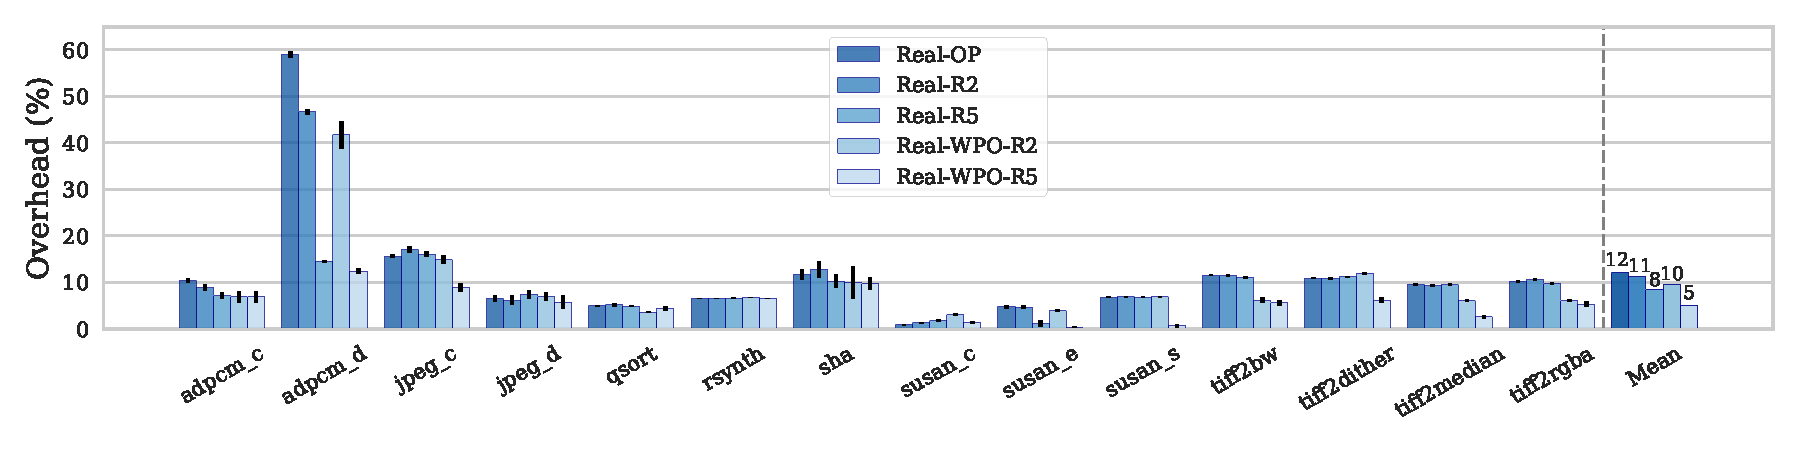
\includegraphics[width=\textwidth]{figs/overhead-O3.pdf}
    \caption{Overhead of the instrumentations compiled with {\flagstype -O3}.}
    \label{fig:overhead-O3}
\end{figure*}

The WPO relaxation was performed using profiling information for every specific input, which provides the perfect information to perform the WPO relaxation.
This means that the experiments show its best performance enabled by having perfect profiling information.

%\begin{figure*}[ht]
%    \centering
%    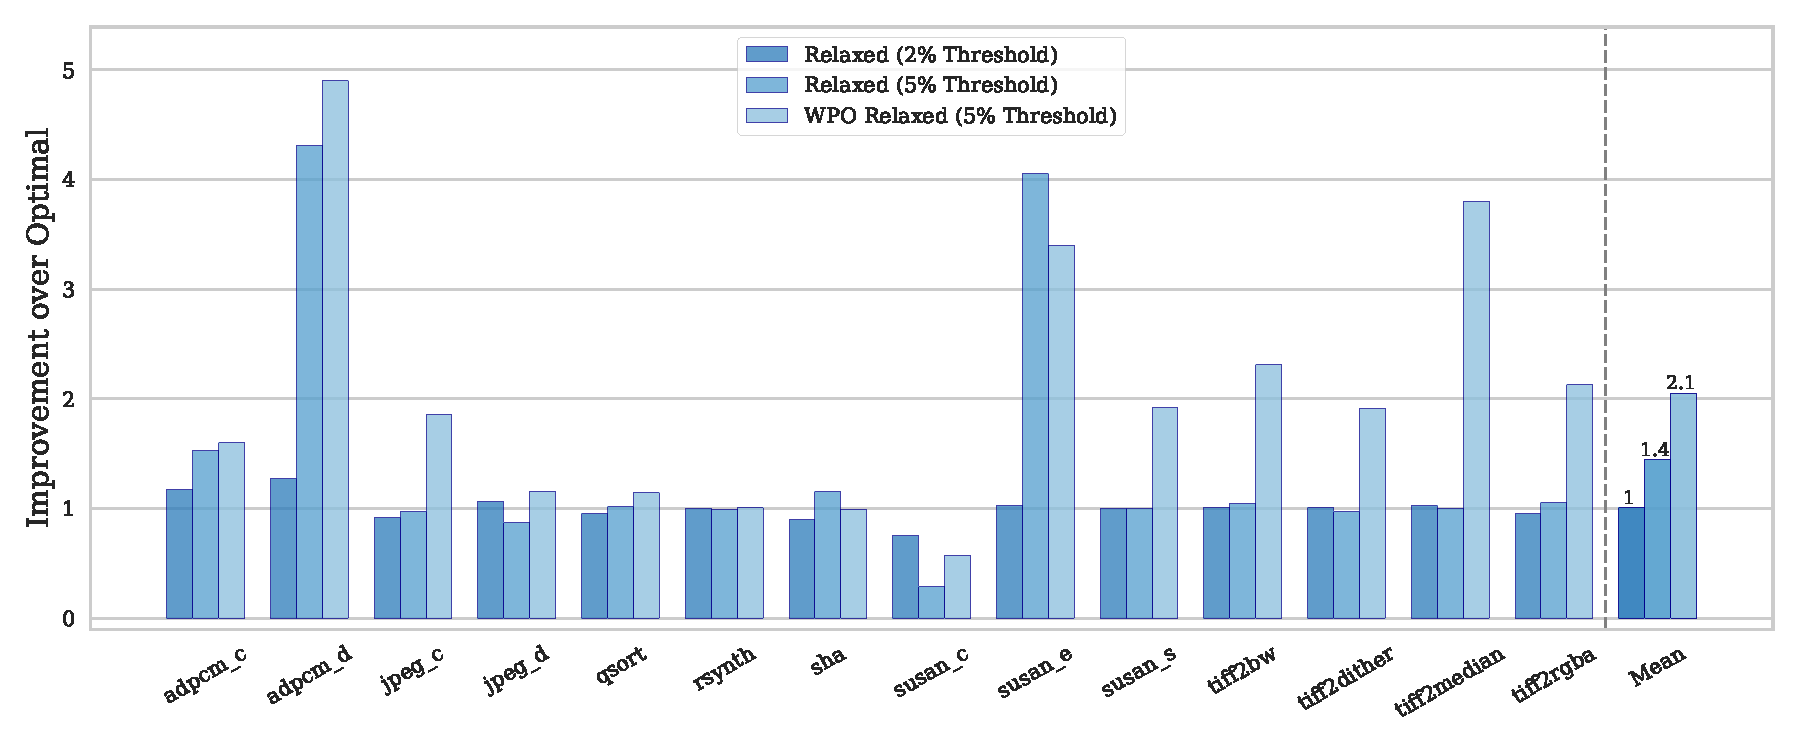
\includegraphics[width=\textwidth]{figs/overhead-improvement-O3.pdf}
%    \caption{Overhead of the instrumentations compiled with {\flagstype -O3}.
%             Notice that the average of the ratios does not equal the ratio of the averages.}
%    \label{fig:overhead-improvement-O3}
%\end{figure*}

\begin{figure*}[h!]
    \centering
    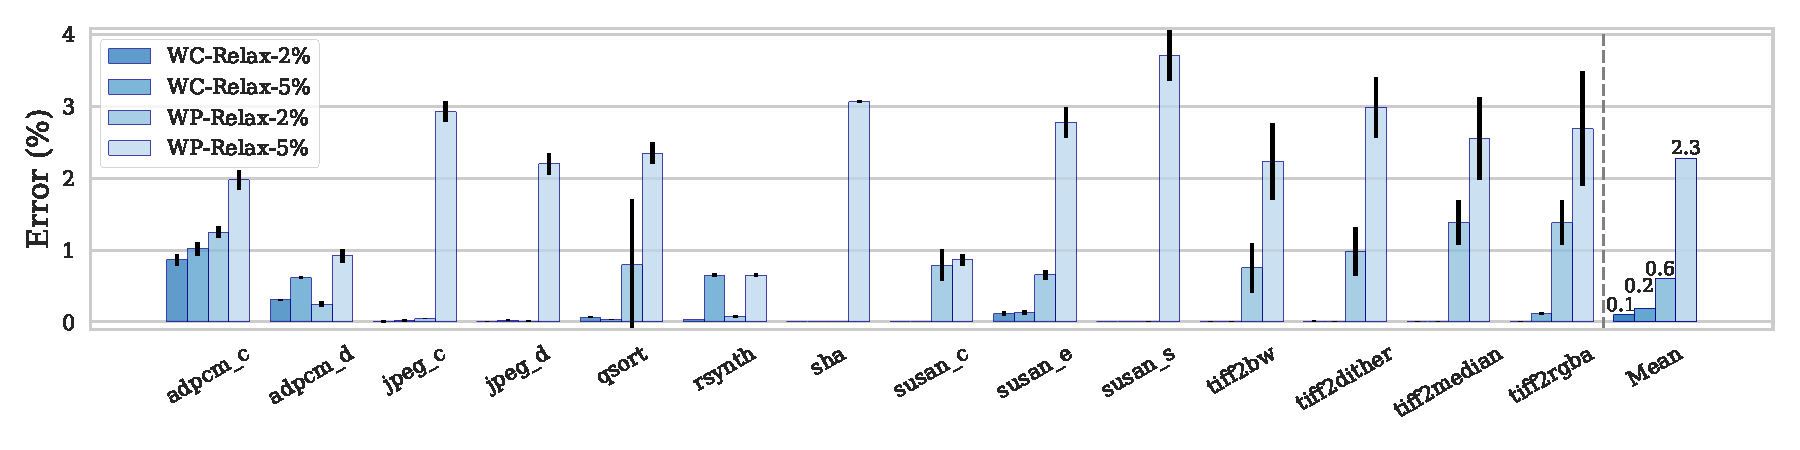
\includegraphics[width=\textwidth]{figs/error-O3.pdf}
    \caption{Dynamic error of the work profiling averaged over the 1000 inputs, after relaxing the number of probes.}
    \label{fig:error-O3}
\end{figure*}

%Figure~\ref{fig:overhead-improvement-O3} shows that the relaxation algorithm, with 5\% threshold, is able to improve an average of 48\% over the optimal instrumentation,
%and the WPO relaxation achieves an average of $2\times$ improvement over the optimal instrumentation.
%While the optimal profiling has a maximum overhead of almost 60\%, the work profiling with a relaxation of 5\% threshold has an overhead of less than 20\% for all benchmarks,
%with the WPO relaxation reaching an average overhead of only 5\%, compared to an average of 12\% for the optimal profiling.

Furthermore, these improvements can be obtained while incurring very little dynamic error, as shown in Figure~\ref{fig:error-O3}.
This result confirms the overly conservative aspect of the relaxation algorithm applied per DAG,
while the WPO relaxation is significantly less conservative.
Because we performed the WPO relaxation having perfect profiling information, its dynamic error was always below the 5\% thresholds.
Although it is not guaranteed by the algorithm, profiling representative inputs should also result in small dynamic errors.

\subsection{Evaluation of the Online {\IterComp}}

For comparison, we use four configurations\footnote{A configuration using the WPO relaxation was not used due to the time necessary for executing the experiments.}.
In all configurations, the same optimization sequence is used for multiple inputs, using a dynamic input-window size, as explained in Section~\ref{sec:oic-infra}.
The average performance over the input window provides an estimate for the overall performance of the optimization sequence across distinct inputs.
The optimization sequences are ranked based on their average performance, and the best optimization sequence is selected.
%When selecting the best optimization sequence, they are ranked by the average of their performance measurement, using the WP metric, except for the Oracle-RM which uses the real speedup over \texttt{-O0}.
\begin{itemize}
\item \textbf{Oracle-RM} executes the program multiple times for each input, measuring the real speedup for each optimization sequence, and then uses the real speedup over {\flagstype -O0} for comparing the optimization sequences.
  The speedups are computed based on the wall-clock time.
  In order to reduce noise, the program is executed several times for the same input, until the confidence interval was no larger than 1\% for a 99\% confidence.
\item \textbf{Oracle-PP} represents an oracle with a \textit{perfect} non-intrusive profiling.
  Although it uses the WP metric for comparing optimization sequences, this oracle also avoids noise in its measurements by also executing the program multiple times for each input.
  The first execution is used for profiling the work metric.
  The remaining executions are used for measuring the wall-clock time without using the work profiling.
\item \textbf{Real-OP} corresponds to the online {\itercomp} as it would be applied in a real online scenario.
  For each optimization, a random sample of inputs is selected, and the program is executed only once with each input.
  When executing each input, it uses the optimal work instrumentation for profiling the work metric.
  The average of the WP for the sample of inputs is then used for selecting the best optimization.
\item \textbf{Real-R5} is similar to the {Real-OP}.
  It also corresponds to the online {\itercomp} as it would be applied in a real online scenario.
  For each optimization, a random sample of inputs is selected, and the program is executed only once with each input.
  When executing each input, it uses the relaxed work instrumentation, with a 5\% threshold, for profiling the work metric.
  The average of the WP for the sample of inputs is then used for selecting the best optimization.
\item \textbf{Real-IPC} corresponds to the online {\itercomp} based on the IPC metric.
  For each optimization, a random sample of inputs is selected, and the program is executed only once with each input.
  The average of the IPC metric for the sample of inputs is then used for selecting the best optimization.
\end{itemize}
The comparison between Oracle-RM and Oracle-PP is useful for validating the use of the WP metric for guiding {\itercomp}, while the other configurations demonstrate the viability of applying the online {\itercomp} in a real scenario.

Figure~\ref{fig:window-size} shows the average input-window size for each benchmark and configuration.
It shows that we can have a statistically sound measurement of the performance metric using just a small number of inputs.

\begin{figure*}[htb]
    \centering
    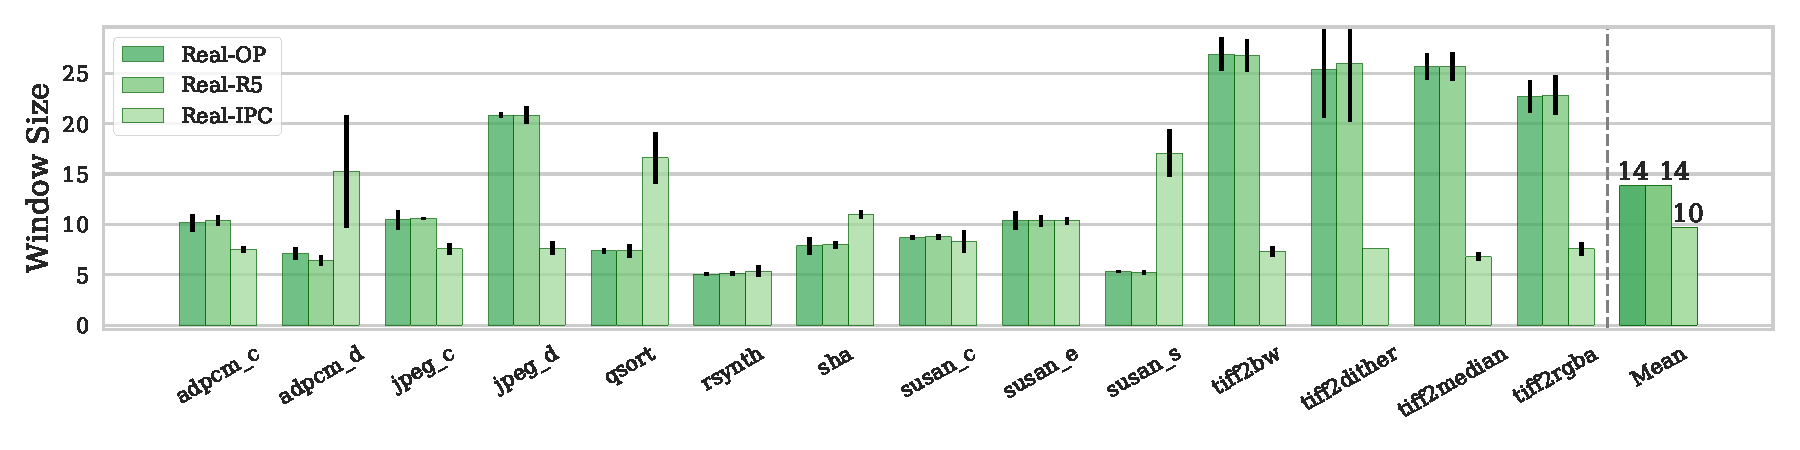
\includegraphics[width=\textwidth]{figs/window-size.pdf}
    \caption{Average input-window sizes observed during the online {\itercomp}.}
    \label{fig:window-size}
\end{figure*}

\subsection{The Set of Optimization Sequences}

For the purpose of evaluating the use of the WP metric with {\itercomp}, we collected in advance a fixed set of optimization sequences.
The reason for using this fixed set, as explained in Section~\ref{sec:oic-infra}, is because this paper is focused on other components of the infrastructure for performing {\itercomp} and we assume that a good generator of optimization sequences will be used in a real online scenario.
This set contains 500 optimization sequences collected in a random search using the training benchmarks.
These optimization sequences contain an average of 40 individual optimization passes, including repetitions, with a maximum of 119 optimization passes, but it also contains optimization sequences which consist of a single flag, such as the default optimizations {\flagstype -O1}, {\flagstype -O2}, {\flagstype -O3}, {\flagstype -Os}, and {\flagstype -Oz}.

  % \begin{minipage}{0.9\textwidth}
  %    \vspace{1em}
  %    \noindent\textbf{Example of a short optimization sequence:}\vspace{-1ex}
  %    \justify{\flagstype -mem2reg -simplifycfg -constprop -dce}
  % \end{minipage}
  %
  % \begin{minipage}{0.9\textwidth}
  %    \vspace{1em}
  %    \noindent\textbf{Example of a long optimization sequence:}\vspace{-1ex}
  %    \justify{\flagstype -globalopt -reassociate -instcombine -loop-rotate -block-freq -deadargelim -early-cse -sroa -argpromotion -sccp -tbaa -barrier -constmerge \mbox{-loop-vectorize} -domtree -basicaa -memdep -basiccg -memcpyopt \mbox{-constprop} -adce -globaldce -mem2reg -constmerge \mbox{-globaldce} -constprop -instsimplify -dse -dce -simplifycfg -loop-unroll -reassociate -constprop \mbox{-globaldce} -instsimplify -adce -constmerge -bb-vectorize -dce -mergefunc -simplifycfg -dse -loop-unroll -globaldce}
  % \end{minipage}
  %
  % \begin{minipage}{0.9\textwidth}
  %    \vspace{1em}
  %    \noindent\textbf{Example of an optimization sequence which includes {-O3}:}\vspace{-1ex}
  %    \justify{\flagstype -O3 -adce -globaldce -simplifycfg -memcpyopt -reassociate -mergefunc \mbox{-dce} -dse}
  %    \vspace{2em}
  % \end{minipage}

Repeating the same optimization pass can be beneficial and usually expected by other passes.
For example, the {\flagstype -loop-simplify} pass is used for transforming loops into a canonical form by inserting pre-header and exit basic blocks.
Although this pass inserts jumps due to redundant basic blocks, this canonical form can be favourable to other loop optimizations.
Because of the redundant basic blocks, this optimization pass expects that the {\flagstype -simplifycfg} will eventually be executor later on the optimization pipeline.
Another example of such inter-relation between transformations concerns the {\flagstype -licm} and {\flagstype -mem2reg} passes.
The {\flagstype -licm} pass is responsible for moving invariant code out from the loop body.
It usually creates new local variables, using memory access operations, for assisting with the code manipulation, which means that the executing the {\flagstype -mem2reg} pass afterwards would be useful as a cleanup pass for removing the extra memory accesses generated.
However, many of the analysis required for identifying loop invariant also benefit from the transformations performed by the {\flagstype -mem2reg} pass.
These examples illustrate the importance of repeating optimization passes.
Moreover, they illustrate the intricate relation amongst several transformations.

However, all optimization sequences in the set of optimizations were generated completely at random, without using any knowledge of individual transformations.
Each optimization sequence was generated in two steps: \textit{(1)} randomly selects the number of flags; \textit{(2)} randomly selects the flags, allowing repetitions.
Afterwards, this randomly generated optimization sequence would be included in the set of optimization sequences only if it was able to improve the performance of a training benchmark, also selected at random, in respect of the {\flagstype -O3} default optimization.
This process was repeated until we obtained all the 500 distinct optimization sequences.

\subsection{Performance Evaluation}

In order to evaluate the quality of the final optimization sequences selected by the {\itercomp} search, we compare their speedup by measuring wall-clock time of the benchmarks when compiled with the standard {\flagstype -O3} optimization.
For each benchmark, after selecting the final optimization sequence, we compute the average speedup over all the 1000 input dataset.
When measuring the wall-clock time for each input, to reduce noise, we execute the same input until we have a statistically sound measurement, i.e. we execute until we have an interval no larger than 1\% with 99\% confidence.
Figure~\ref{fig:speedups} shows these average speedups over all the 1000 input dataset.
This figure shows that the best optimization sequence selected with the Oracle-PP is very close to the performance of the best optimization sequence selected with the Oracle-RM.
This result is important for demonstrating that a work-based metric has the potential to produce good results in a real online scenario, where there is the restriction that programs execute distinct inputs only once.
Moreover, the evaluation also indicates that the use of relaxation algorithms does not degrade the optimization search,
it might even benefit the {\itercomp} as it tends to insert smaller interferences in the performance measurement.
Finally, Figure~\ref{fig:speedups} also presents the results of {\itercomp} guided by IPC, which is futher discussed in Figure~\ref{fig:ipc-vs-work}.

\begin{figure*}[htb]
    \centering
    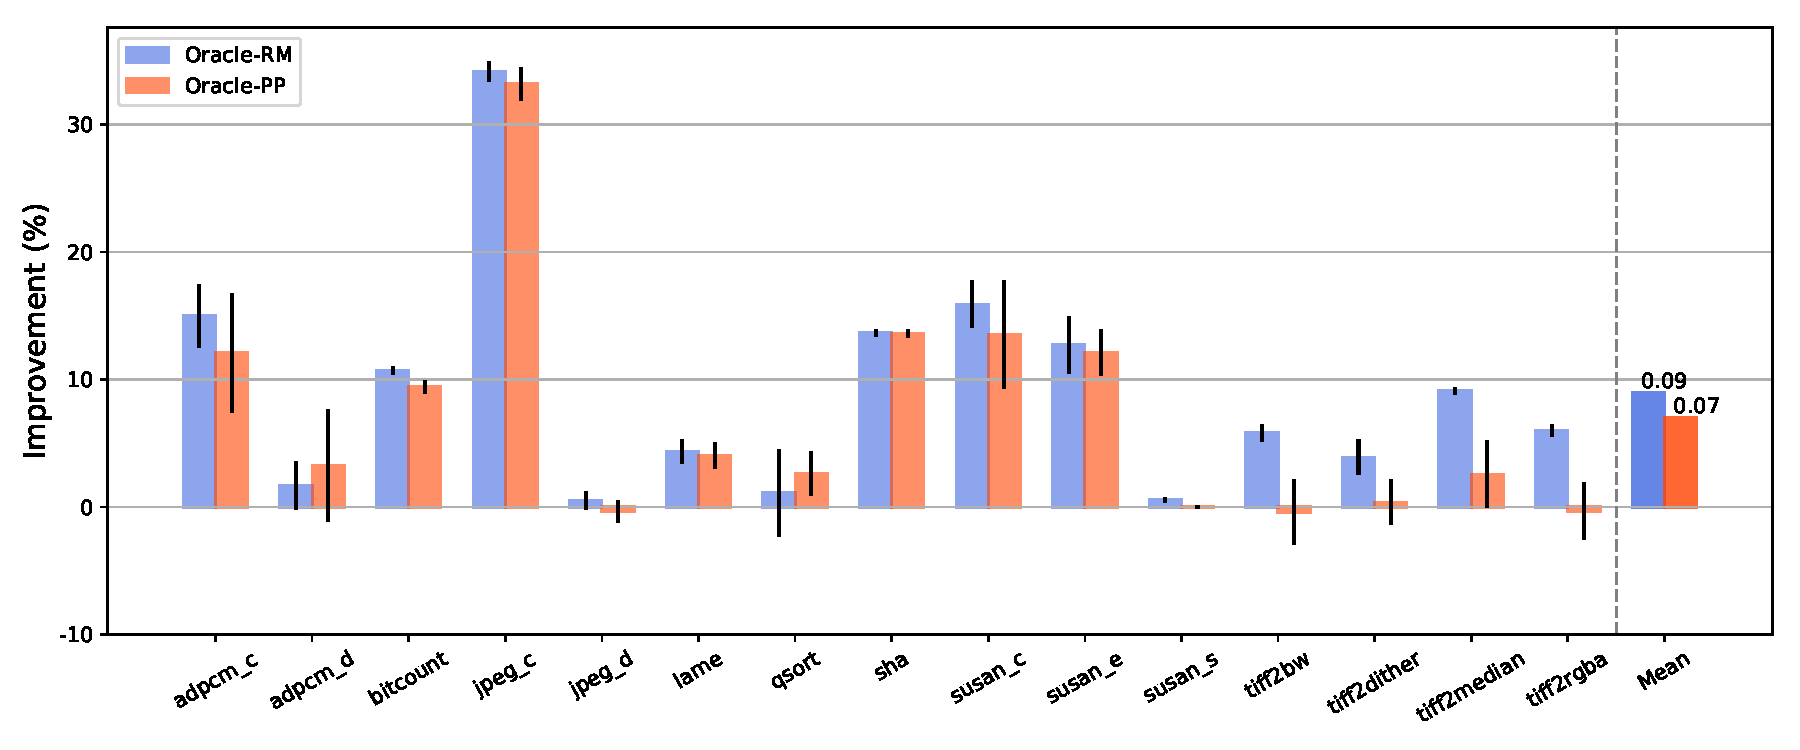
\includegraphics[width=\textwidth]{figs/speedups.pdf}
    \caption{Speedups obtained from the final optimization sequence selected by the online {\itercomp}.
	         The speedups reported for each benchmark represents the average speedup across their complete 1000 input datasets.}
    \label{fig:speedups}
\end{figure*}

%\begin{figure*}[h]
%    \centering
%    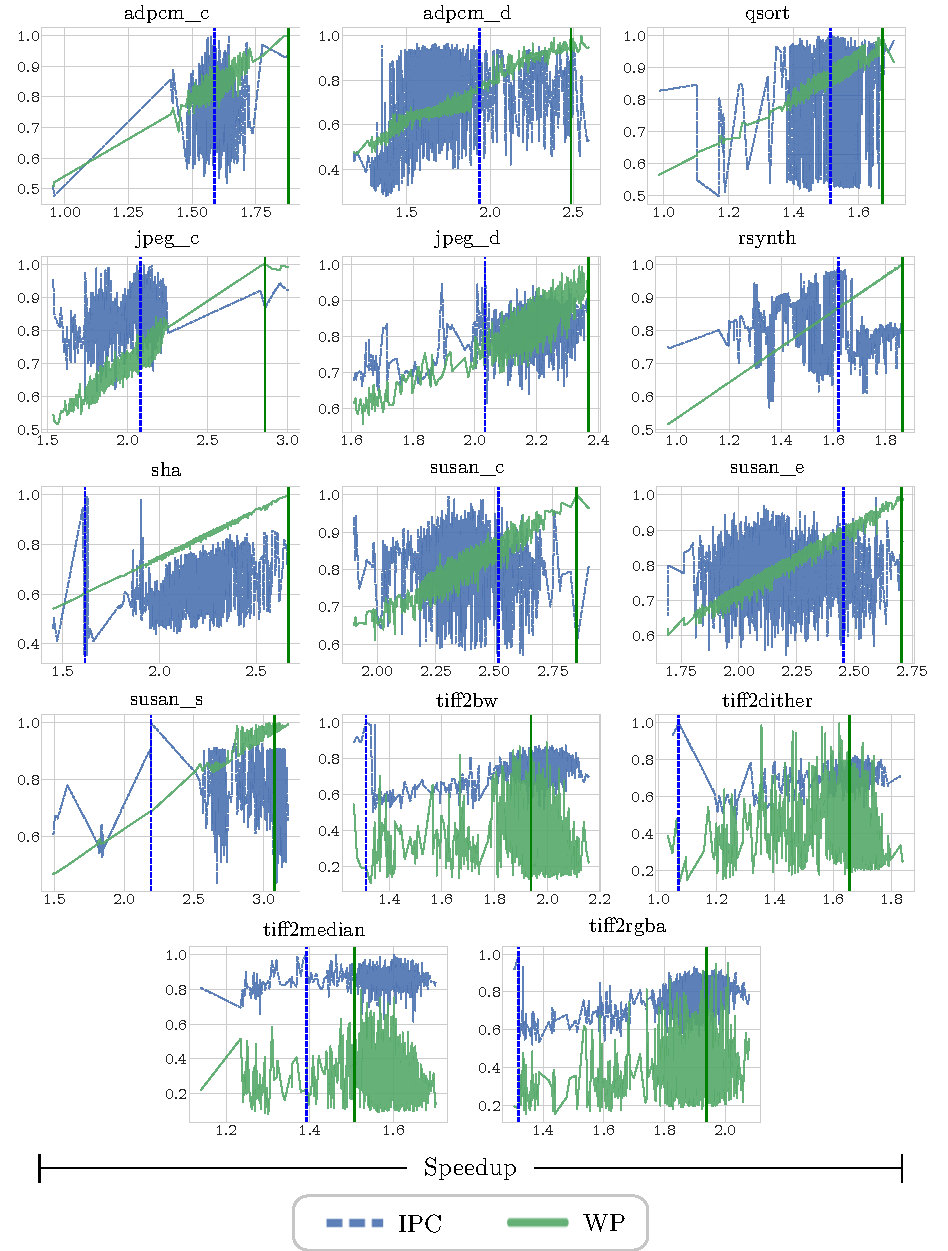
\includegraphics[width=\textwidth]{figs/ipc-vs-work.pdf}
%    \caption{Comparison between {\itercomp} using IPC or the WP metric.}
%    \label{fig:ipc-vs-work}
%\end{figure*}

%Figure~\ref{fig:ipc-vs-work} presents a comparison between IPC and the WP metric regarding their correlation with the actual speedup over \verb|-O0| observed during {\itercomp}.
%Each point in the figure corresponds to each metric averaged over input windows collected during multiple executions of the {\itercomp}.
%The vertical lines correspond to the optimization sequence selected by the {\itercomp} search, which either represents the highest IPC or the highest value of WP.
%In all cases, the optimization sequence selected based on the WP is much closer to the best speedup than the optimization sequence selected based on IPC, which can be attributed to the fact that the WP has a stronger correlation with the speedup.
%In all cases, IPC shows little to no correlation with the speedup, which corroborates the argument given in Section~\ref{sec:ipc-vs-work-metric}.

%For some cases, namely for the tiff-related benchmarks, the WP shows a worse correlation with speedup.
%We believe these cases could be improved by improving the cost model used to compute the work metric.
%However, even in these cases, the optimization sequences selected based on the WP outperform those selected based on the IPC metric.

\textbf{ToDo: Include results using Genetic Algorithm search.}
